\documentclass[margin]{res}
\usepackage{graphicx}
\usepackage{tabu}
\usepackage{multirow}

%\usepackage{helvetica} % uses helvetica postscript font (download helvetica.sty)
%\usepackage{newcent}   % uses new century schoolbook postscript font 
\setlength{\textwidth}{5.1in} % set width of text portion
\renewcommand{\arraystretch}{1.2}

\begin{document}

% Center the name over the entire width of resume:
 \moveleft.5\hoffset\centerline{\Large\bf Aarsh Verdhan}
% Draw a horizontal line the whole width of resume:
 \moveleft\hoffset\vbox{\hrule width\resumewidth height 1pt}\smallskip
\hskip-3.0cm\begin{tabular*}{6in}{l@{\extracolsep{\fill}}r}
        & \multirow{1}{*}{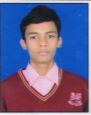
\includegraphics[scale=1]{profile}}\\
         
        %-----------------------------------------------------------  
        House no 733, Tuglakabad& \\
        New Delhi-110044  \\
        Delhi\\
        averdhen123@gmail.com \\
        8920403086\\
    \end{tabular*}
 \section{OBJECTIVE} To obtain an internship that will help me to explore new horizons in the field of computer science.\\

\section{EDUCATION}\begin{tabu} to 1\textwidth { | X[c] | X[c] | X[c] | X[c]| X[c]|}
 \hline
 Degree & College /School & University & Passing Year & Pass Percentage\\
 \hline
 BTech. & Delhi Technological University & Delhi Technological University & 2021 & 8.2 (Till Sem III) \\
\hline
HSC & Sahoday Sr. Sec. School   & CBSE & 2017 & 94.0\\

\hline
SSC & Sahoday Sr. Sec. School   & CBSE & 2015 & 9.8 CGPA\\

\hline
\end{tabu}
\section{PROJECTS } \begin{enumerate}
 \item  {\large{\sl Pollinator Bee EYRC-2018}}\\
        - Implemented various control algorithms such as PID using ROS (Python).\\
        -Implemented various Object detection algorithms using OpenCV (Python).\\

  \item  {\large{\sl Autonomous Underwater Vehicle}}\\
Worked on the software part of the Autonomous Underwater Vehicles "ARYA 1.0" and "VARUNA 2.0"\\
        - Implemented various object localization algorithms using OpenCV (C++) and Deep Learning.\\
        -Developed the control stack for the communication of rosnodes using ROS(C++).\\
\item {\large{\sl 3D Reconstruction of Stereo images}}\\
 Developed a system to generate 3D coordinates of a point from stereo images.\\
  	-Implemented a camera callibrator to get the camera matrix.\\
	-Implemented the algorithms of pose estimation and depth mapping.\\
	-Built using OpenCV in python.\\
\item {\large{\sl Wallpaper Changer to Spotlight Images (Windows)}}\\
 Developed a software to change windows wallpaper to spotlight images.\\
  	-Implemented file handling.\\
	-Implemented the OS library of pyhton.\\
	-Built using python.\\
\item {\large{\sl Using Mobile Phone to collect IMU and Camera data}}\\
 Developed a software to obtain IMU and Camera feeds from a phone using Roslibjs.\\
  	-Built using javascript.\\
\item {\large{\sl Created a chrome extension to manipulate Youtube}}\\
 Developed a chrome extension to manipulate youtube eg. skipping ads faster.\\
  	-Built using javascript.\\
\item {\large{\sl Developed an Android app "Anonytter" as anonymous twitter}}\\
 Developed an android app to post anonymous tweets.\\
  	-Built using java and XML.\\
\item {\large{\sl Developed an Image Classifier using MNIST dataset}}\\
 implementation done using Keras.\\
  	-Built using Python.\\
\item {\large{\sl Built DTU-AUV website}}\\
 
  	-Built using Express and MongoDB\\
\item {\large{\sl Manipulated TurtleSim movement with input signs}}\\
 
  	-Built using ROS\\

\item {\large{\sl Sudoku Solver from image}}\\
 
  	-Built using OpenCV and trained MNIST dataset\\
\section{RESEARCH AND PUBLICATIONS } 
 
\section{    }

\section{    }
\section{    }


\section{TRAINING AND INTERNSHIPS} \begin{itemize}
 
 \item{\sl  "Machine Learning" course by Coding Ninjas }
 \item{\sl  "Competitive programming " course by Coding Ninjas}
 \item{\sl  "intro to Nodejs" course by Udacity}
 \end{itemize}

\section{TECHNICAL  \\ SKILLS} \begin{enumerate}
\item {\sl Programming Langauges \& Scripts }\\
	-Python, Nodejs, JavaScript, C/C++
\item {\sl Algorithms \& Data Structures }\\
\item {\sl Frameworks \& Libraries}\\
	-Tensorflow, Opencv, Keras, matploitlib, Pandas, Bootstrap, Express, Django, ROS (Robot Operating System)
\item {\sl Web Technologies}\\
	-ExpressJs ,MEAN,HTML5, CSS3, Information Retrieval 
\item{\sl Databases}\\
	-MongoDB,MySQL
\end{enumerate}



\section{SOFT SKILLS }\begin{enumerate}
\item{\sl Fast Decision Making }
\item{\sl Perseverance}
\item{\sl Patience}
\item{\sl Taking Responsibilities and Leadership role}
\end{enumerate}

\section{EXTRA CURRICULAR ACTIVITIES}\begin{itemize}
\item{\sl Secured top 68 ranks in CBSE writing series, 2015}
\item{\sl Secured 3rd rank at DTC writing series, 2015}

\item{\sl Participated at SAUVC-2017, Singapore}

\item{\sl Participated at NIOT-2018, Chennai}
\item{\sl Participated at IEEE Extreme, 2018}
\end{itemize}

\section{CO CURRICULAR ACTIVITIES}\begin{itemize}
\item{\sl Participated in various interschool speech and debate competitions}
\item{\sl Participated in various quiz competitions}
\end{itemize}


\section{PERSONAL INFORMATION}
{\sl Father's Name:} Anand Verdhan\\
{\sl Mother's Name:} Rita Kumari\\
{\sl Sex:} Male\\
{\sl Date of Birth:} 22nd November 1998\\
{\sl Nationality:} Indian\\
{\sl Maritial Status:} Unmarried\\

\section{DECLARATION} 
{\sl I here by declare that the above information is true and best of my knowledge}

 \section{DATE}
 {\sl : 17th April 2019}
%-----end



	\end{enumerate}


\end{document}